\section{Materials \& Methods}

When species remain in ecological contact over evolutionary time, the nature of their interaction may leave distinctive signatures in their phylogenies. \cite{bastolla2009architecture} Most of the literature on the topic addresses the co-diversification in one of two ways, depending on the initial assumptions. One may begin without the assumption co-diversification has occurred, and then ascertain the likelihood that it did. Or, having established that co-diversification has occurred either by testing for it or through some other piece of exogenous evidence, one may ascertain what history is most likely. The first approach yields an overall likelihood, and the second yields a sequence of events (host switches, extinctions and bifurcations) that may have resulted in the observed associations.

We are interested in learning about the natural history of the system, and so we would like to ask a somewhat enlarged question. {\em In a system where the hosts are associated with a very large number of guest clades, which guest clades show evidence of co-diversification with the hosts?}

\subsection{Phylogenetic signal and trait-based approaches}

For each organism that appears among the microbiomes of a group of hosts, there exists a pattern of observed associations between the ``guest'' organism and the host organisms. These associations can be treated as traits of the host, and the history of each association can be examined like any phenotypic trait. Alternatively, the tendency to associate (or not) with a host could be treated as a trait distributed over a group of microbial organisms, although it is difficult to imagine how one might demarcate the boundaries between groups. Association with a particular host is more likely to correspond to different traits for more distantly related bacteria, and so it is probably not meaningful to naively apply stochastic trait mapping across all bacterial diversity.

In {\em Analysis of phylogenetics and evolution with {\tt R}} (p. 236), Emmanuael Paradis describes phylogenetic signal as follows :

\begin{quote}
The concept of phylogenetic signal is at the heart of most phylogenetic methods. From a statistical point of view, a phylogenetic signal is defined by the non-null covariances (i.e., non-independence) among species. From a biological point of view, phylogenetic signal is a direct consequence of the evolution of traits and its form will depend on the evolutionary mechanisms in action.
\end{quote}

The advantage of this approach is that it decomposes the problem into a large number of smaller problems. Every OTU (operational taxonomic unit) is treated as an independent trait, and observed associations are simply plugged into one of the four established models. All of them have been implemented in {\tt R}. Unfortunately, this is also a key disadvantage. Most trait-based models do not account for interactions {\em among} traits, or a way to account for traits that have their own evolutionary model, independent of the organisms that exhibit them. 

A second disadvantage of trait-based approaches when applied to co-diversifying systems arises from the non-uniform distribution of microbial diversity with respect to 16S diversity. Individual OTUs may represent several organisms, each with their own pattern of association (Figure \ref{fig:FP_fig4}). Comparing phylogenetic signal among different OTUs thus depends on the diversity underlying each of the OTUs. Correcting for this would require a relatively complete and unbiased survey of microbial diversity.

\subfile{FishPoo/figures/figure4}

\subsection{Tests for cospeciation}

Hafner {\em et al.} \cite{hafner1994disparate} examines the relationship between pocket gophers and their chewing louse parasites. This paper addresses there first question using a tree reconciliation test implemented in {\tt COMPONENT} by Roderic D. M. Page \cite{page1993genes}. It is, in essence, a parsimony approach; the gene duplication and loss events necessary to achieve topological congruence between two trees are minimized. Hafner {\em et al.} first reject the null hypothesis (independent evolution) by applying the tree reconciliation test among gopher, louse and randomly drawn trees, and then examine rates of nucleotide divergence between the gopher and louse. 

This dataset has since been reanalyzed in many other publications, has become a sort of base-case for co-diversification methods. Notably, Huelsenbeck {\em et al.} introduced the use of Bayesian inference to cospeciation \cite{huelsenbeck2000bayesian}.

Hommola {\em et al.} \cite{hommola2009permutation} describe a method to extend the Mantel test. \cite{mantel1967detection} The Mantel test is a statistic on the correlation of two matrixes, and requires that the matrixes be of equal rank. When applied to distance matrixes for trees containing differing numbers of taxa, one must delete or duplicate taxa until the matrix ranks are equal. This results in anomalous results which Hommola {\em et al.} explore in detail. To address this issue, they take every pair of linked tips (e.g., a parasite species that is observed to associate with a host species), and examine the correlation of distances through the two trees. This accommodates trees of arbitrary size and arbitrary patterns of association among their tips, and can be coupled with a straightforward permutation test to estimate the significance of the correlations. One can walk through every clade in the phylogeny of host-associated OTUs and, for every clade, compute the Hommola correlation with the host phylogeny (Figure \ref{FP_hommola_corr}). 

\subfile{FishPoo/figures/figure5}

However, there are some important difficulties when it comes to applying the Hommola cospeciation test to a large number of clades belonging to the same tree. Fist of all, this approach necessarily entails multiple comparison, and so a correction to the significance values is required. However, a Bonferroni correction is not appropriate because the structure of each clade is not independent of the others. Rather, they are hierarchically nested within a tree, which is itself inferred from an probabilistic model (an approximate maximum likelihood model, in this case), which is based on nucelotide transitions inferred from from an alignment. The autocorrelation within the tree would need to be accounted for, but calculating it would not be straightforward. At a minimum, one would need to take into account the fact that the multiple comparisons have hierarchical relationships.

The second difficulty arises from the need to perform unsupervised correlation tests. Hommola {\em et al.} use the Pearson product-moment correlation, which assumes that the processes are independent, identically distributed, and follow a bivariate normal distribution. Unfortunately, there is reason to suppose that the distances among tips of a phylogenetic tree would be normally distributed. Of course, other correlation statistics could be substituted at the expense of computational complexity (Spearman's rank correlation coefficient, for example, obeys quadratic scaling), but the number of OTUs present in a typical microbiome would call for the use of a supercomputer.

\subfile{FishPoo/figures/figure6}

The reliance on a summary statistic likely dooms the application of Hommola {\em et al} as a way to detect co-diversification in the microbiome, where a supervised method is not practical. All summary statistics are a form of information reduction, usually a projection into a 1-dimensional space, and their interpretation depends on structural properties within the data. While it is often possible to construct complimentary tests to insure that assumptions hold, those tests are themselves likely to rely on summary statistics. Ultimately, someone has to actually inspect the data. \cite{anscombe1973graphs} For example, compare the distribution of pairwise distances for the Gopher/Louse dataset \cite{hafner1994disparate} to Clade 72223, which appears just below it in Figure \ref{FP_highcorr}. Both have about the same correlation coefficient ($r=0.490$ verses $r=0.488$), very high significance ($1.38\times 10^{-9}$ verses $p=3.21\times 10^{-223}$ and are within an order of magnitude in size ($15 \times 17$ verses $14 \times 68$). Nevertheless, the two distributions are obviously different, and the vertical banding pattern in Clade 72223 is strongly reminiscent of Case 4 in Anscombe's quartet. The structural differences between these interactions can also be seen clearly when represented as tanglegrams (Figure \ref{fig:FP_tangles}).

\subfile{FishPoo/figures/figure7}

In principle, one could develop a hierarchical Bonferroni correction, design correlation tests that exclude artifactual features that crop up in distributions of patristic distances, and obtain the use of a powerful supercomputer. However, a third difficulty remains. All of the approaches mentioned so far are based upon an idealized model of co-diversification. In the ideal case, the host and the guest organisms would diverge in lockstep and exhibit phylogenies of perfectly congruent structure. One might imagine this to be the case for vertically transmitted symbionts, but the reality is that it is not even true for different genes within the same organism (MDM: cite some ILS papers here, like some of Graham Coop's). Indeed, many of the methods used to study co-diversification were originally developed with the aim of reconciling gene trees into species trees(MDM: and cite some more). Real cases of co-diversification can be expected to manifest along with other effects, such as ecological interactions with organisms that do not belong to either clade, stochastic variations in nucleotide divergence, extinctions, sampling bias and the emergence of cryptic species. The model, and the statistical tests applied to it, must be able to distinguish between a real case with deviations arising from these other processes and a spurious or artifactual resemblance to one. If the effect of competing processes were small, one could apply the a stringent statistical cutoff. Unfortunately, this is not the case. As mentioned before, the Gopher/Louse dataset from Hafner {\em et. al.} exhibits a Hommola correlation of $r=0.49$, which is rather poor as correlated processes go. Nevertheless, the ecological case for cospeciation is solid and its physiological basis is sound. The Sedge/Smut interaction from Escudero \cite{escudero2015phylogenetic} is also well established, but has a Hommola correlation of only $r=0.15$. It would not make sense to search for new cases of co-diversification with a method that only works within a statistical stringency that would exclude all known cases of the effect. It is possible to address this problem by including other processes in the model, but each new parameter also introduces additional risk of overfitting.

\subsection{Specimen collection and housing}

Specimens were purchased through the aquarium trade and housed in a vivarium on at UC Davis under the supervision of M.D.M and P.C.W. Specimens were housed in single-species groups within 30-100L aquaria filtered by air-driven sponge filters.

\subfile{FishPoo/figures/figure1}
\subfile{FishPoo/tables/table1}

%\begin{figure}
%    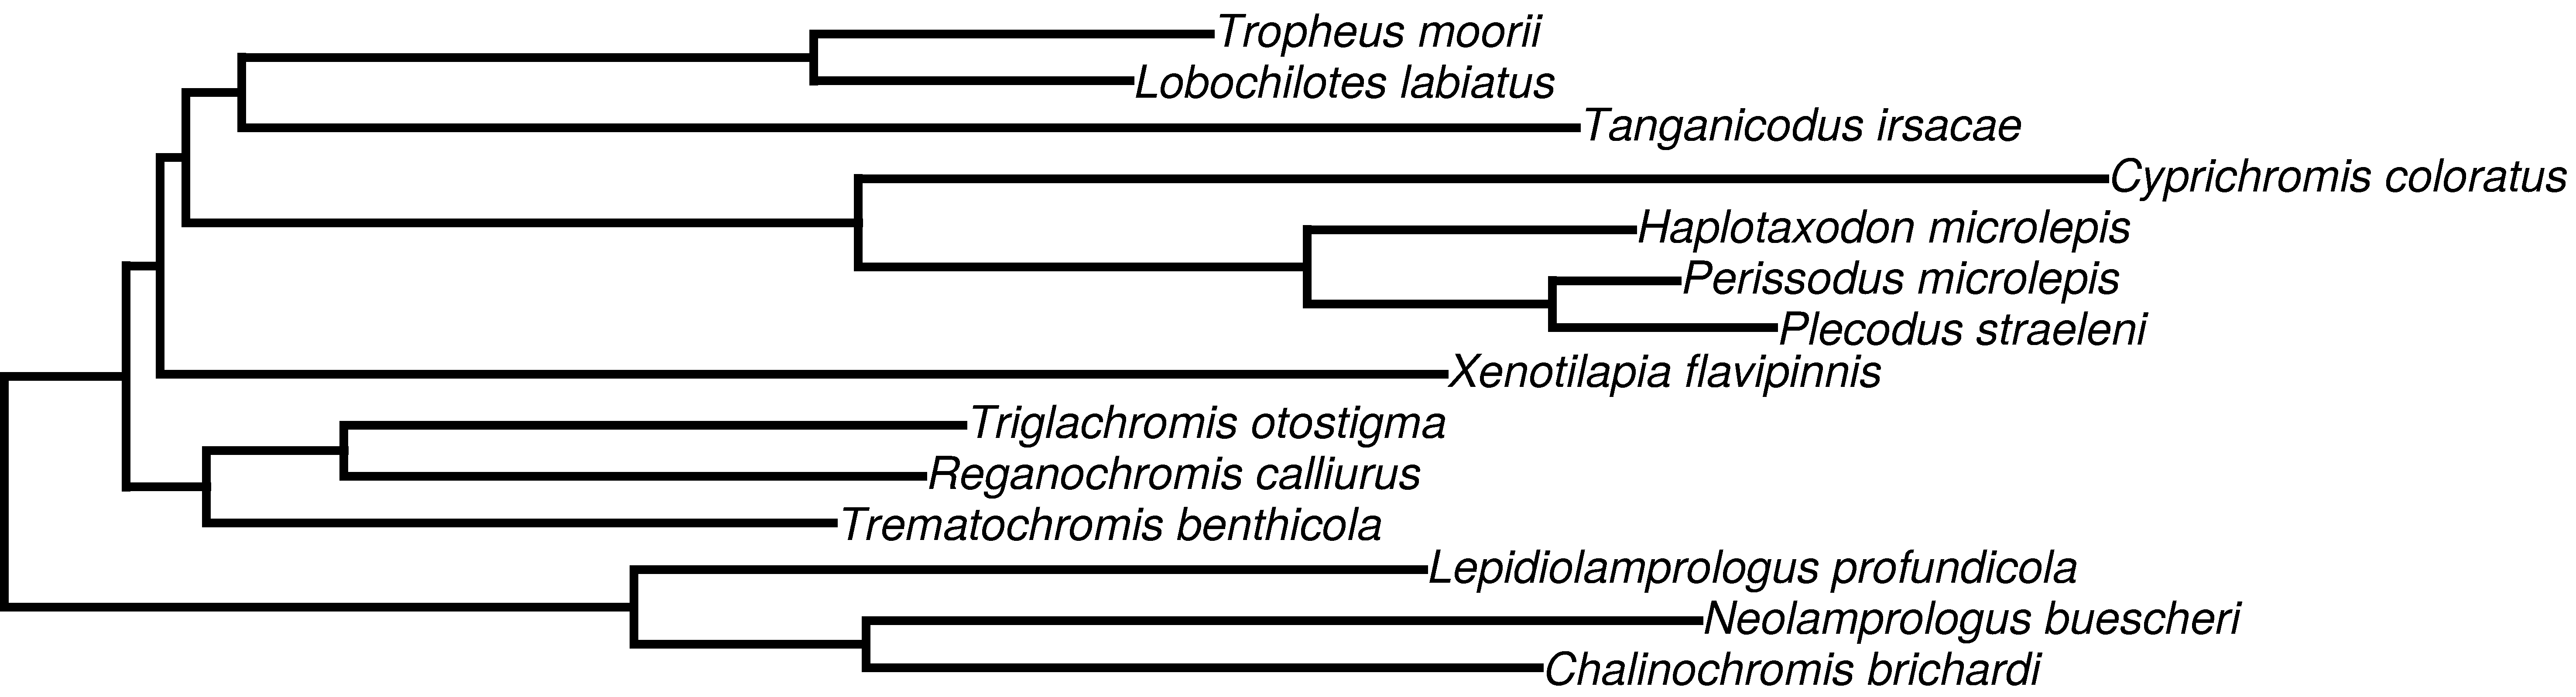
\includegraphics[width=\textwidth]{FishPoo/figures/mcgee_tree.pdf}
%    \caption{A maximum likelihood phylogeny of the host organisms.}
%    \label{FP_host_tree}
%\end{figure}

\subfile{FishPoo/figures/figure2}

\subsection{Sample collection}

Specimens were fed until satiated and placed into 30L tanks. To minimize microbial contamination in the water and tank silicone, we lined each tank with a sterile autoclave bag prepared with 10 liters of molecular water augmented with a small amount of sodium chloride and calcium chloride. To minimize potential contamination from biological filtration, we used chemical filtration via sterile charcoal pellets to sequester nitrogenous wastes produced by the fish, and a sterile plastic tube was submerged and connected to an air pump to aerate the water. Stool was removed using a sterile serological pipette and frozen. Fish remained in these tanks for less than 24 hours and were then returned to their original aquarium.

\subsection{Sample preparation, processing and sequencing}

Stool samples were subjected to bead beating for 60 seconds and DNA was extracted using MoBio PowerSoil DNA Isolation kit in accordance with the manufacturer's protocol. DNA was amplified by a two-step PCR enrichment of the V4 region of the 16S rRNA gene using primers 515F and 806R, modified by addition of Illumina adaptor and barcodes sequences. Libraries were sequenced using an Illumina MiSeq system, generating 250 base pair paired-end amplicon reads. The amplicon data was multiplexed using dual barcode combinations for each sample. A custom script available in a GitHub repository (\url{https://github.com/gjospin/scripts/blob/master/Demul_trim_prep.pl}), to assign each pair of reads to their respective samples when parsing the raw data. This script allows for one base pair difference per barcode. The paired reads were then aligned and a consensus was computed using {\tt Trimmomatic} \cite{bolger2014trimmomatic} with maximum overlap of 120 and a minimum overlap of 70 (other parameters were left as default). The custom script automatically demultiplexes the data into {\tt fastq} files and parses the results to reformat the sequences in {\tt fasta} format.

\subsection{Building the observation table}

Chimera were identified with {\tt vsearch}, \cite{rognes2016vsearch} and unique reads were identified using {\tt hat-trie}. \cite{askitis2005cache, askitis2007hat} A table of observation counts were constructed as a {\tt Pandas} {\tt DataFrame} object, \cite{mckinney2010data} and a count threshold was applied. Tables of raw counts and normalized counts were written as comma separated value files, and the corresponding sequences were written as a FASTA file. All analysis was carried out and documented in Jupyter Notebooks \cite{perez2007ipython} and visualizations, including all those appearing in this manuscript, were constructed using {\tt Matplotlib}. \cite{hunter2007matplotlib}

\subsection{Building phylogeny of OTUs}

The Illumina sequencing platform has a substitution error frequency of about 0.1\%. \cite{ross2013characterizing} Trimming and filtering reads based on quality score removes about 69\% of substitution errors, on average, \cite{schirmer2016illumina} and overlap correcting paired-end reads improves this to about one substitution error in every 14 reads. \cite{bolger2014trimmomatic} At the sacrifice of sensitivity, the error frequency can be reduced arbitrarily by excluding very rare sequences. For example, excluding sequences observed only once reduces the substitution error frequency to about one in every 200 sequences. Most substitution errors are likely to be corruptions of sequences already present in the data, and so phylogenetic reconstruction should place them as sister leafs of their uncorrupted sources. This confines the effect of substitution errors to the smallest topological scale, where it appears in the form of ``extra'' leafs that are randomly attached with the minimum branch length.

Alignment of the observed sequences is performed using {\tt Clustal Omega}, \cite{goujon2010new, sievers2011fast} and an approximate maximum likelihood phylogeny is constructed using {\tt FastTree}. \cite{price2009fasttree, price2010fasttree}

%\begin{figure}
%    \includegraphics[width=\textwidth]{FishPoo/figures/fishpoo_tree.png}
%    \caption{An approximate maximum likelihood phylogeny of the guest organisms.}
%    \label{FP_guest_tree}
%\end{figure}

\subfile{FishPoo/figures/figure3}

\subsection{Spectral analysis and machine learning}

Classifying organisms by how long they have been present in a particular habitat can yield insights regarding their origins, especially when these relationships are repeated in many similar but distinct habitats. Phylogeographic models regard this collection of habitats as the nodes of a meta-community network. The edges of this network represent dispersal rates, a convolution of both the vectors of dispersal and the barriers that impinge on those vectors. Organisms move from habitat to habitat in discrete events with probabilities related to the dispersal rates. If organisms are gathered from each habitat, and trees of related organisms are constructed, these trees may be used to infer the rates of dispersal. These rates reveal, at least in broad strokes, the structure of the relationships among the habitats.

The host tree and guest tree are loaded as {\tt SuchTree} objects, and linked together through the observation table as a {\tt SuchLinkedTrees} object. The {\tt SuchTree} class allows for extremely rapid traversals of large trees, enabling distance correlations to be efficiently computed. The {\tt SuchLinkedTrees} class leverages this to compute graph adjacency and graph Laplacian matrixes of subtrees of host and guest phylogenies. Spectral decomposition and kernel densities of graph Laplacians are computed using {\tt numpy}, and the Jensen-Shannon divergence is calculated between each pair of spectral densities using the {\tt entropy} function in {\tt scipy.stats}. \cite{walt2011numpy} Feature tables were assembled using {\tt Pandas} \cite{mckinney2010data} and machine learning was carried out using {\tt scikit-learn}. \cite{pedregosa2011scikit}

\subsection{Correlation-based analysis}

For each clade of guest organisms, the {\tt SuchLinkedTrees.linked\_distances} function is used to calculate the pairwise distances through the host and guest trees for every pair of non-null observations in the link matrix, as described by Hommola {\em et al.} \cite{hommola2009permutation} The Pierson's correlation for these distances is computed using the {\tt pearsonr} function from {\tt scipy.stats}. \cite{walt2011numpy}

\subsection{Literature search for comparative analysis}

Trees and interaction matrixes were compiled from the supplementary material from Rezende {\em et al.}, \cite{rezende2007non} Hafner {\em et al.} \cite{hafner1994disparate} and Escudero \cite{escudero2015phylogenetic} for a total of fifty data sets (Table \ref{FP_studies_table}). Synthetic interactions with perfect phylogenetic congruence and with no phylogenetic congruence were simulated using {\tt Dendropy}. \cite{sukumaran2010dendropy} NEEDS DETAIL ON SIMULATIONS